\documentclass{article}

% ICML 2026 style. Place icml2026.sty, icml2026.bst and fancyhdr.sty in this directory
% (from the official icml2026.zip) before compiling on Overleaf.
\usepackage{microtype}
\usepackage{graphicx}
\usepackage{booktabs}
\usepackage{amsmath}
\usepackage{amssymb}
\usepackage{multirow}
\usepackage{url}
\usepackage[hidelinks]{hyperref}
\newcommand{\theHalgorithm}{\arabic{algorithm}}

\usepackage[accepted]{icml2026}

%% ===================================================================
%% EDIT THIS ONE LINE with your GitHub repository URL before submitting.
\newcommand{\repourl}{https://github.com/pruthav23/CHE629_Optimus5Prime}
%% ===================================================================

\icmltitlerunning{Beyond Optimus 5-Prime: Chemistry-Conditioned and Attention-Augmented 5'UTR Models}

\begin{document}

\twocolumn[
\icmltitle{Beyond Optimus 5-Prime: Chemistry-Conditioned, Attention-Augmented, and\\
Interpretable Models of 5$'$UTR Translation Control}

\begin{icmlauthorlist}
\icmlauthor{Tushar Srikrishna Sridhar (231103)}{iitk}
\icmlauthor{Anika Gupta (230137)}{iitk}
\icmlauthor{Prutha Vinay (230807)}{iitk}
\end{icmlauthorlist}

\icmlaffiliation{iitk}{Indian Institute of Technology Kanpur, Kanpur, India}
\icmlcorrespondingauthor{Tushar Srikrishna Sridhar}{tsridhar23@iitk.ac.in}

\icmlkeywords{5'UTR, translation, mean ribosome load, convolutional networks, attention, variant effect prediction}

\vskip 0.3in
]

\printAffiliationsAndNotice{}

\begin{abstract}
The 5$'$ untranslated region (5$'$UTR) of a messenger RNA controls how efficiently that
message is translated, which makes it a central design variable for mRNA therapeutics.
\citet{sample2019} introduced \emph{Optimus 5-Prime}, a convolutional network that predicts
mean ribosome load (MRL) from a 50\,nt 5$'$UTR and explains 93\% of the variance of a
massively parallel reporter assay. We reproduce that result from scratch in PyTorch~\citep{paszke2019}
($r^2=0.919\pm0.006$ over three seeds), first validating the whole pipeline on a
\emph{synthetic} dataset whose generative rules we control, and we benchmark the model
against three alternatives under one shared protocol. We then address four limitations of
the original work. (i) A single chemistry-conditioned model with shared trunk and
per-chemistry heads replaces three separate networks and improves the modified-nucleotide
chemistries ($\Psi$ $+0.012$, m1$\Psi$ $+0.020$ $r^2$) while transferring markedly better
across chemistries. (ii) A systematic architecture $\times$ data-regime study shows a
CNN+attention hybrid reaching $r^2=0.942\pm0.001$, clearly above the published CNN, while a
pure transformer fails outright in low-data regimes. (iii) Pre-training on unmodified RNA
and fine-tuning on only 1{,}000 $\Psi$ sequences recovers 95\% of full-data performance.
(iv) Attribution analysis recovers the Kozak-context upstream-AUG motif \emph{de novo} and
shows that the hybrid learns the same grammar as the CNN. We also report two clear negative
results: a Siamese paired model does not beat simple subtraction for variant-effect
prediction, and we do not reproduce the paper's claim that secondary structure matters more
for modified chemistries. Code, trained weights and all per-run metrics:
\url{\repourl}.
\end{abstract}

\section{Introduction}
\label{sec:intro}

Translation of a eukaryotic mRNA begins when the small ribosomal subunit binds near the
5$'$ cap and scans along the transcript until it recognises a start codon. Everything the
scanning ribosome encounters before the main coding sequence (CDS) therefore shapes how much
protein the message yields: upstream AUG codons (uAUGs) that capture scanning ribosomes,
upstream open reading frames (uORFs) that terminate before the CDS, the Kozak sequence
context around each start codon, and secondary structure that impedes scanning~\citep{kozak1986}. The 5$'$UTR
is thus a compact, highly interpretable regulatory element, and one that can be engineered:
tuning a 50\,nt sequence is a practical lever for mRNA vaccine and therapeutic design.

\citet{sample2019} made this problem tractable for machine learning. They built a massively
parallel reporter assay (MPRA) over a library of 280{,}000 random 50\,nt 5$'$UTRs, measured
the \emph{mean ribosome load} (MRL) of each by polysome profiling, and trained a
three-layer convolutional network, \emph{Optimus 5-Prime}, to predict MRL from one-hot
encoded sequence. The model explains 93\% of held-out variance and generalises to human
5$'$UTRs and to clinical variants.

This report has two halves. First (Sections~\ref{sec:data}--\ref{sec:bench}) we reproduce
the published result and benchmark it, with the discipline that the original paper did not
need: a synthetic dataset with known ground truth to validate the pipeline before touching
real data, and a single protocol applied identically to every model. Second
(Section~\ref{sec:novelty}) we extend the work along four axes that correspond to four
limitations of the original: separate models per RNA chemistry, a single architecture
evaluated only at full data, a weak subtraction-based variant-effect procedure, and
largely uninterpreted convolutional filters.

\paragraph{Contributions.}
\begin{enumerate}\itemsep2pt
\item A faithful PyTorch reproduction ($r^2=0.919\pm0.006$ vs.\ 0.93 published), verified by
loading the authors' own Keras weights into our implementation ($r^2=0.934$).
\item A synthetic 5$'$UTR simulator with known rules and a computable noise ceiling, used to
validate the pipeline and to test \emph{which} rules each model actually learns.
\item A three-benchmark comparison under one protocol, reporting regression and
classification metrics (accuracy, macro precision/recall/F1, confusion matrices).
\item Four extensions: a chemistry-conditioned multi-task model, an architecture $\times$
data-regime study yielding a hybrid that beats the published CNN, a cross-chemistry transfer
study, and an attribution/motif analysis. Two extensions produce negative results, which we
report in full.
\end{enumerate}

\section{The Original Work}
\label{sec:paper}

\paragraph{Biological problem.} Given a 50\,nt 5$'$UTR immediately upstream of a fixed
reporter CDS, predict how heavily ribosomes load onto that transcript. MRL is a scalar
summary of the polysome distribution: transcripts are fractionated by the number of bound
ribosomes, and
$\mathrm{MRL} = \sum_{k} k \, p_k$,
where $p_k$ is the fraction of that UTR's reads in polysome fraction $k$. High MRL means
efficient translation initiation.

\paragraph{Dataset.} A library of random 50-mers was cloned upstream of eGFP, transcribed
\emph{in vitro}, transfected into HEK293T cells, and separated over a sucrose gradient into
14 fractions, each sequenced. After filtering, the 280{,}000 most deeply sequenced UTRs were
retained. The authors also produced the same library with uridine replaced by pseudouridine
($\Psi$) or N1-methylpseudouridine (m1$\Psi$) --- the modified nucleotides used in mRNA
vaccines~\citep{kariko2008} --- an mCherry-CDS library, a designed library containing 35{,}212 human 5$'$UTRs
and 3{,}577 ClinVar variants, and a variable-length (25--100\,nt) library.

\paragraph{Deep learning formulation.} Each UTR is one-hot encoded to a $50\times4$ matrix.
Optimus 5-Prime applies three 1-D convolutions (120 filters, width 8, \texttt{same} padding,
ReLU), flattens, and passes through a 40-unit dense layer with 20\% dropout to a single
linear output. It is trained with MSE on standardised MRL using Adam ($10^{-3}$), batch 128,
for three epochs --- the authors stop there because the model begins to overfit. Performance
is reported as $r^2$, the \emph{squared Pearson correlation} between observed and predicted
MRL on the 20{,}000 most deeply sequenced UTRs, which are held out.

\paragraph{Related work.} \citet{karollus2021} later extended this line of work with a
frame-aware pooling layer that handles 5$'$UTRs of arbitrary length; our hybrid is
complementary, keeping the fixed 50\,nt input of the original but changing how positions are
combined.

\section{Data and Experimental Setup}
\label{sec:data}

\subsection{Real data and splits}
We use GEO accession GSE114002. Following the original protocol exactly, UTRs are sorted by
total read count, the top 280{,}000 are kept, the \textbf{top 20{,}000 form the test set},
and the remaining \textbf{260{,}000 form the training pool}. Because deeper sequencing means
less measurement noise, this makes the test set the cleanest part of the data; we therefore
also report a random-split control (Section~\ref{sec:arch}).

The published recipe has no validation set: it fixes three epochs. For every experiment
beyond the literal reproduction we carve a validation split from the training pool
(10\% at full data, 20\% in small-data regimes) and use it for \emph{all} model selection ---
learning rate, dropout, and early stopping. The 20{,}000 test UTRs are never used for any
choice, and training subsets are drawn only from the training pool. Subset indices and seeds
are saved to disk.

An important data detail: the $\Psi$ and m1$\Psi$ files store 59\,nt per row (the 50\,nt UTR
plus 9\,nt of CDS). Trimming to the first 50\,nt is required for the sequences to match the
unmodified library; without it the overlap is zero. After trimming, 19{,}968 of the 20{,}000
test UTRs carry labels in all three chemistries, which gives a shared test set for
cross-chemistry comparison.

\paragraph{Noise ceiling.} Because two biological replicates exist per chemistry, the best
$r^2$ any model can achieve against replicate 1 equals the Pearson correlation between
replicates: 0.971 (U), 0.916 ($\Psi$), 0.865 (m1$\Psi$). These bound every number we report.

\subsection{Synthetic dataset}
\label{sec:synth}
The paper's library is often called ``synthetic'', but only the \emph{sequences} are
designed; the MRL labels are real measurements with real noise. To validate our pipeline
before using real data, we built a genuinely synthetic dataset of 280{,}000 random 50-mers
with labels generated from rules we control, following a leaky-scanning model:
\begin{equation}
\mathrm{MRL}_{\text{true}} = 1 + 7 \cdot e^{0.025\,\mathrm{MFE}} \prod_{i \in \mathcal{A}} (1 - r_i),
\end{equation}
where $\mathcal{A}$ is the set of upstream AUGs and $r_i = b_i \cdot \kappa_i$. The base
repression $b_i$ depends on what the uAUG does: 0.40 if an in-frame stop precedes the CDS
(a self-contained uORF, permitting reinitiation), 0.75 if it is out of frame with no stop
(an overlapping ORF), and 0.12 if it reads in frame into the CDS (an N-terminal extension).
The Kozak factor $\kappa_i = 0.35 + 0.35\,[\,-3 \in \{A,G\}\,] + 0.30\,[\,+4 = G\,]$.
Minimum free energy (MFE) is computed with ViennaRNA~\citep{lorenz2011}. Observed labels add
$\mathcal{N}(0, 0.45^2)$, which fixes a computable noise ceiling of $r^2 = 0.918$.

This dataset serves three purposes: it validates preprocessing and training code against a
known answer; it bounds achievable performance; and, because we know the planted rules, it
lets us ask \emph{which} rules a model has learned rather than only how well it scores.

\section{Reproduction}
\label{sec:repro}

\begin{figure}[t]
\centering
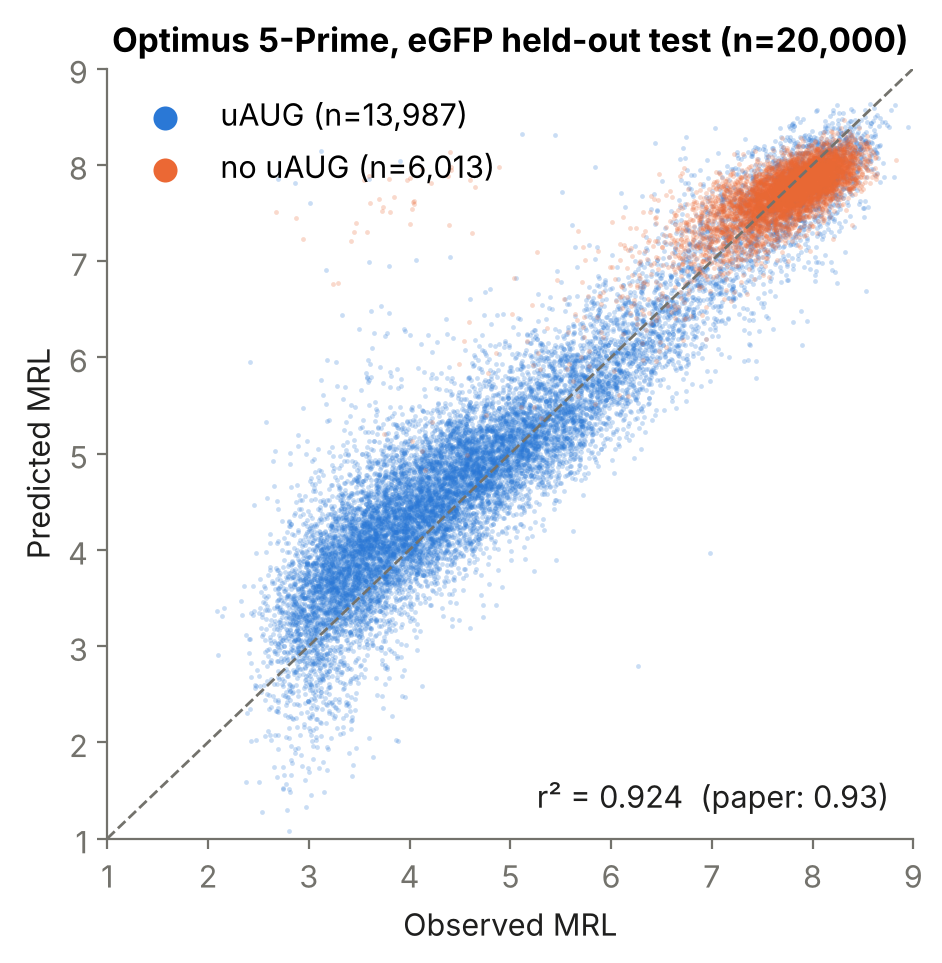
\includegraphics[width=\columnwidth]{figs/fig2b_test_scatter.png}
\caption{Reproduction of the paper's Figure~2b. Predicted vs.\ observed MRL on the 20{,}000
held-out UTRs, coloured by presence of an upstream AUG. Our from-scratch model reaches
$r^2=0.924$ on this seed (published: 0.93). The uAUG-free sequences (orange) occupy the
high-MRL mode, as expected biologically.}
\label{fig:repro}
\end{figure}

\paragraph{Pipeline validation.} Before training anything, we loaded the authors' released
Keras weights (\texttt{main\_MRL\_model.hdf5}) into our PyTorch module and evaluated on our
preprocessed test set, obtaining $r^2 = 0.934$. This confirms that our data processing,
one-hot encoding, and architecture match theirs exactly. One subtlety: Keras \texttt{same}
padding for an even kernel ($k=8$) pads 3 on the left and 4 on the right, which must be
replicated for the weights to transfer.

\paragraph{Synthetic first, then real.} On the synthetic dataset the CNN reaches
$r^2 = 0.856 \pm 0.006$ against a noise ceiling of 0.918. Crucially, in-silico insertion of
a single ATG into uAUG-free sequences shows the model recovers the planted rules
quantitatively (Figure~\ref{fig:ism}): mean predicted $\Delta$MRL of $-0.43$ / $-1.38$ /
$-2.39$ for in-frame / uORF / overlapping-ORF insertions, against ground truth $-0.40$ /
$-1.36$ / $-2.52$ ($r = 0.95$ across all insertions). The model has learned the frame logic,
not merely ``ATG is bad''.

On the real data, training from scratch with the published recipe gives
$r^2 = 0.919 \pm 0.006$ over three seeds (0.924, 0.921, 0.910), against the published 0.93
(Figure~\ref{fig:repro}). The residual gap is consistent with seed variance: with only three
epochs, no learning-rate schedule and no early stopping, run-to-run spread is $\approx 0.01$,
and the paper reports a single run. Under our proper train/validation/test protocol with
early stopping the same architecture gives $r^2 = 0.922 \pm 0.002$.

\paragraph{Biological sanity checks.} Independently of the model, the data reproduce the
published frame effect: among single-uAUG UTRs, out-of-frame uAUGs depress MRL to
$\approx 4.5$--$5.5$ while in-frame uAUGs are far milder and approach uAUG-free levels close
to the CDS. We also reproduce the human-UTR evaluation (Figure~4a of the paper) at
$r^2 = 0.784$; the published 0.81 uses a \emph{retrained} model whose weights and exact
recipe are not in the authors' repository. The authors' own original model scores 0.789 on
our pipeline, so the gap is attributable to that missing model rather than to our
implementation.

\begin{figure}[t]
\centering
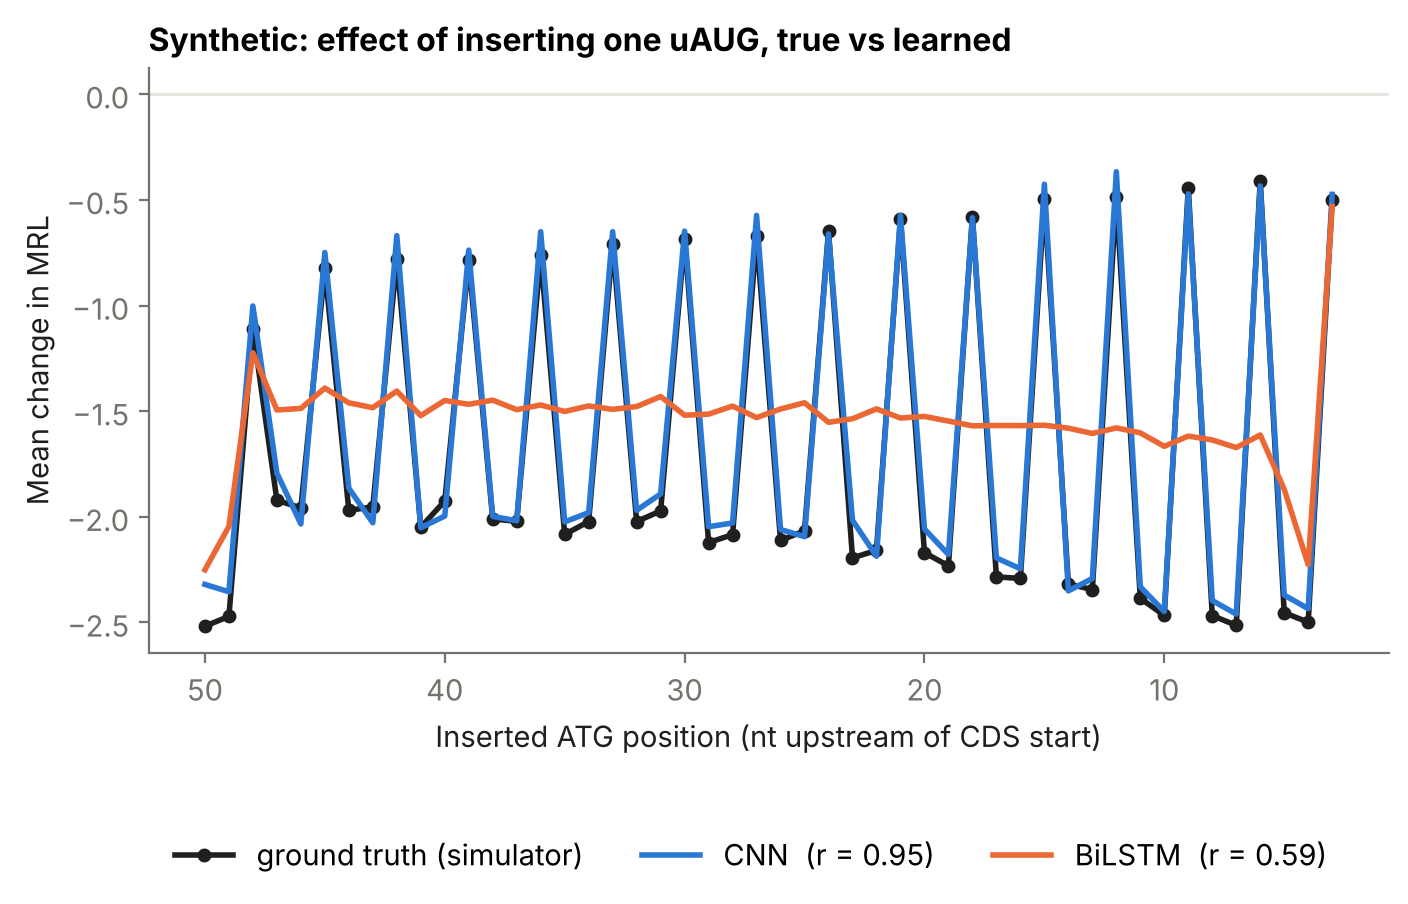
\includegraphics[width=\columnwidth]{figs/synth_atg_insertion.png}
\caption{Rule recovery on synthetic data. A single ATG is inserted at every position of 400
uAUG-free test UTRs and the predicted change in MRL is compared with the simulator's true
change. The CNN tracks the ground truth, including the three-nucleotide frame periodicity;
the BiLSTM learns only that ATG is repressive.}
\label{fig:ism}
\end{figure}

\section{Benchmark Comparison}
\label{sec:bench}

\begin{figure}[t]
\centering
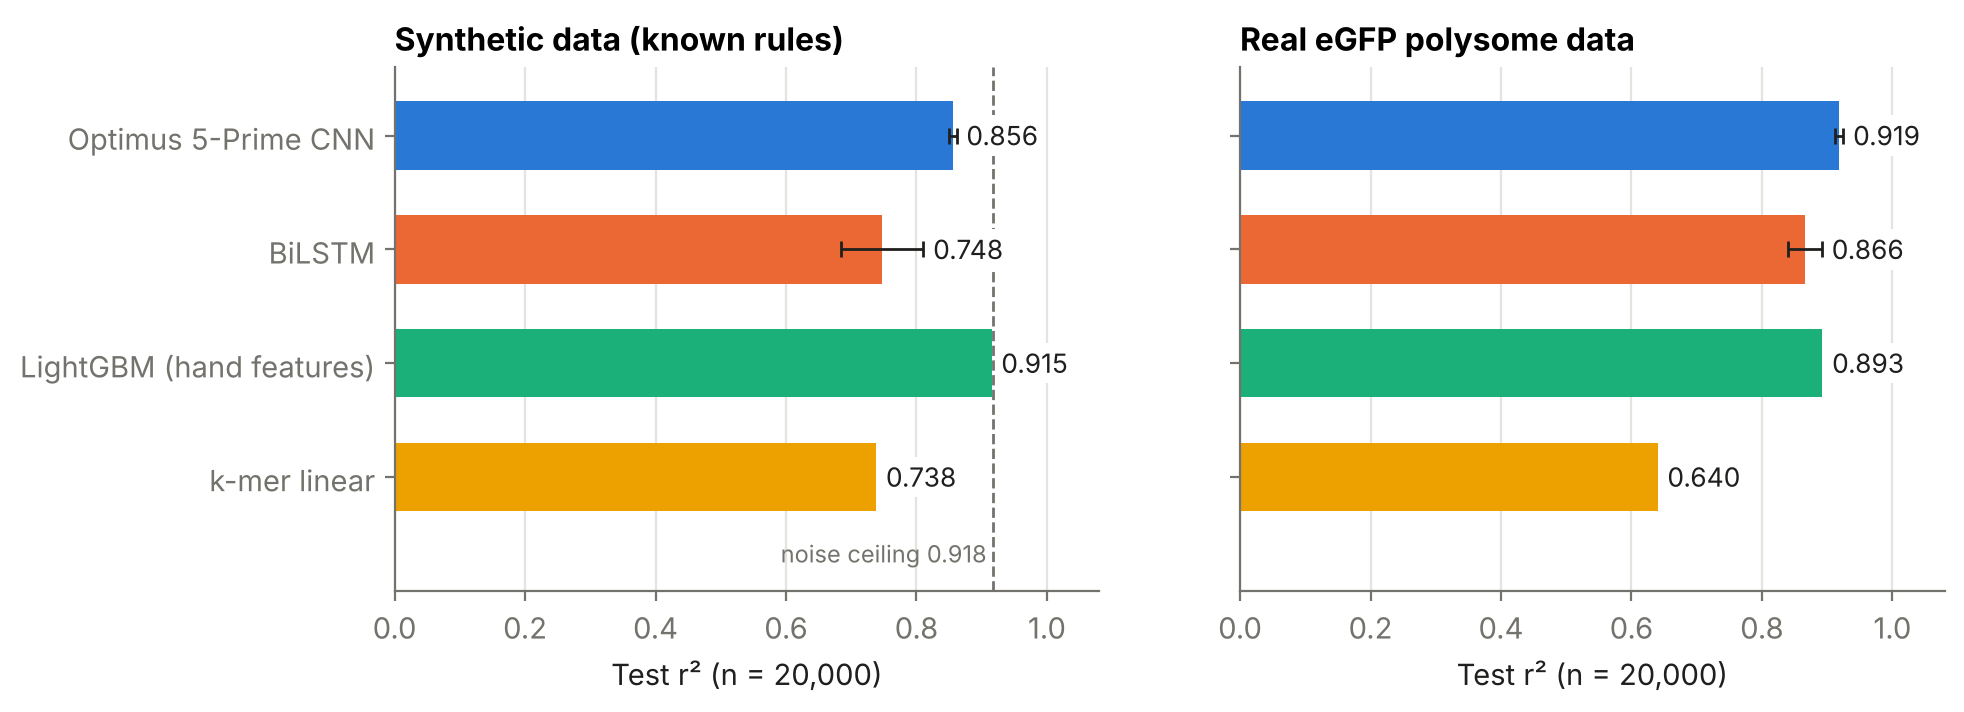
\includegraphics[width=\columnwidth]{figs/r2_synth_vs_real.png}
\caption{Benchmark comparison on synthetic data (left, with computable noise ceiling) and
real eGFP data (right). LightGBM's synthetic score is near-oracle because its hand-crafted
features encode the very rules the simulator plants.}
\label{fig:bench}
\end{figure}

We compare Optimus 5-Prime against three benchmarks, all trained and evaluated under the
identical protocol of Section~\ref{sec:data}:
\begin{itemize}\itemsep2pt
\item \textbf{Position-specific $k$-mer linear model} ($k=1\ldots6$, ridge regression) ---
the paper's own baseline;
\item \textbf{LightGBM}~\citep{ke2017} on hand-crafted features: uAUG counts by functional type, best Kozak
context per type, stop-codon counts per frame, distance of first/last uAUG, GC content, MFE,
and 1--3-mer counts (98 features);
\item \textbf{BiLSTM}~\citep{hochreiter1997} (bidirectional LSTM, mean+max pooling) --- a different deep-learning
family on the same one-hot input.
\end{itemize}

Because the task is regression but the rubric calls for classification metrics, we
additionally bin MRL into \textbf{tertiles of the training distribution} (low $<5.98 \le$
medium $<7.63 \le$ high) and report accuracy and macro-averaged precision, recall and F1,
with confusion matrices. Table~\ref{tab:bench} gives the unified comparison on real data and
Figure~\ref{fig:cm} the confusion matrices; Figure~\ref{fig:bench} contrasts synthetic and
real performance.

\begin{table*}[t]
\caption{Unified comparison on the real eGFP held-out test set ($n=20{,}000$; $n=19{,}968$
for the multi-chemistry rows, which are restricted to UTRs labelled in all three
chemistries). Classification metrics use training-set tertiles of MRL; precision, recall and
F1 are macro-averaged. Mean $\pm$ sd over seeds where more than one seed was run.}
\label{tab:bench}
\vskip 0.1in
\begin{center}
\begin{small}
\setlength{\tabcolsep}{3.4pt}
\begin{tabular}{llcccccccc}
\toprule
Model & Role & Seeds & $r^2$ & Spearman & RMSE & Accuracy & Precision & Recall & F1 \\
\midrule
Optimus 5-Prime CNN & reproduction & 3 & $0.919${\scriptsize$\pm.006$} & 0.942 & 0.547 & 0.869 & 0.822 & 0.822 & 0.819 \\
$k$-mer linear & benchmark & 1 & 0.640 & 0.832 & 1.155 & 0.696 & 0.723 & 0.659 & 0.636 \\
LightGBM (hand features) & benchmark & 1 & 0.893 & 0.922 & 0.620 & 0.848 & 0.795 & 0.791 & 0.791 \\
BiLSTM & benchmark & 3 & $0.866${\scriptsize$\pm.026$} & 0.907 & 0.746 & 0.819 & 0.773 & 0.769 & 0.763 \\
\midrule
Transformer & ours & 3 & $0.728${\scriptsize$\pm.012$} & 0.835 & 1.013 & 0.713 & 0.704 & 0.655 & 0.635 \\
\textbf{CNN + attention hybrid} & ours & 3 & $\mathbf{0.942}${\scriptsize$\pm.001$} & \textbf{0.955} & \textbf{0.454} & \textbf{0.886} & \textbf{0.839} & \textbf{0.843} & \textbf{0.841} \\
Multi-chemistry CNN (U head) & ours & 3 & $0.919${\scriptsize$\pm.007$} & 0.938 & 0.580 & 0.802 & 0.789 & 0.749 & 0.724 \\
\quad + validation recalibration & ours & 3 & $0.919${\scriptsize$\pm.007$} & 0.938 & 0.527 & 0.858 & 0.807 & 0.810 & 0.805 \\
\bottomrule
\end{tabular}
\end{small}
\end{center}
\vskip -0.1in
\end{table*}

\begin{figure*}[t]
\centering
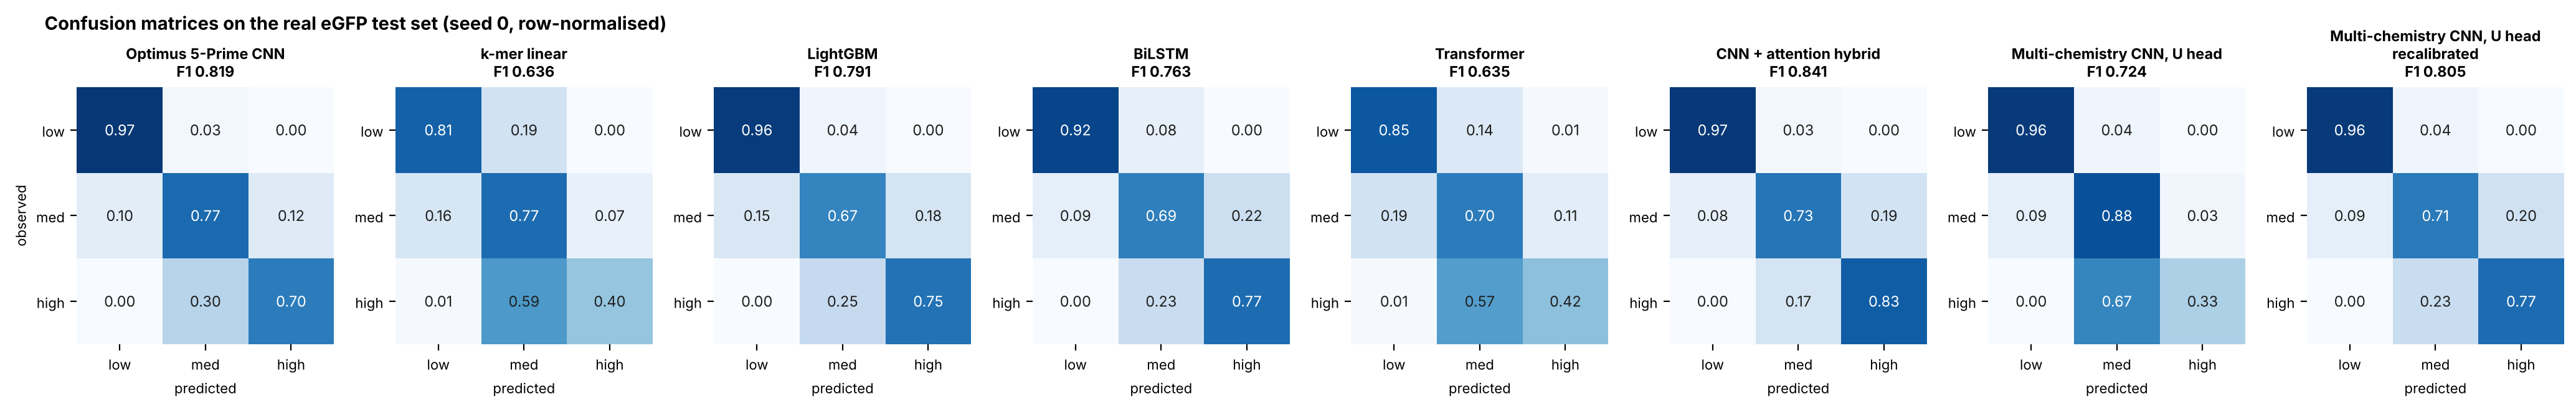
\includegraphics[width=\textwidth]{figs/confusion_matrices.png}
\caption{Row-normalised confusion matrices on the real test set (seed 0) for MRL binned into
training-set tertiles. Every model finds the low-MRL class easiest, because a single uAUG is
a strong and easily learned signal; the high class is hardest, requiring the absence of
repressive elements \emph{and} favourable structure. The uncalibrated multi-chemistry model
(rightmost) illustrates that equal $r^2$ does not imply equal classification quality.}
\label{fig:cm}
\end{figure*}

\paragraph{Interpretation.} Four observations matter more than the ranking itself.

\emph{(i) The deep model earns its place, but not by as much as the paper's baseline
suggests.} The published comparison is against a $k$-mer linear model (0.66 published, 0.640
reproduced here). A properly tuned gradient-boosted model on biologically informed features
reaches 0.893 --- far closer to the CNN. The honest claim is that the CNN beats strong
feature engineering by $\approx 0.03$ $r^2$ while requiring no domain features at all.

\emph{(ii) LightGBM's synthetic score is near-oracle and should not be read as a win.} On
synthetic data it scores 0.915 against the ceiling of 0.918, but its features (uAUG type,
Kozak strength, MFE) are precisely the quantities the simulator uses. This is exactly the
diagnostic value of the synthetic set: it separates ``learned the task'' from ``was handed
the answer''.

\emph{(iii) Classification metrics expose failures that $r^2$ hides.} The uncalibrated
multi-chemistry model matches the single CNN on $r^2$ (0.919) yet scores F1 0.724 vs.\ 0.819,
because its predictions are compressed toward the mean (calibration slope 1.1--1.2) and the
high-MRL class is systematically under-predicted (recall 0.33). A single linear
recalibration fitted on the \emph{validation} split --- never the test set --- restores F1 to
0.805 without changing $r^2$ at all. Reporting only $r^2$, as the original paper does, would
have hidden this entirely.

\emph{(iv) Error structure is biologically sensible.} All confusion matrices are strongly
diagonal with errors confined to adjacent classes; no model confuses low with high MRL. The
low class is recovered best (0.92--0.97 recall for the stronger models), consistent with a
single out-of-frame uAUG being a near-deterministic repressive signal.

\section{Extensions}
\label{sec:novelty}

\subsection{A chemistry-conditioned multi-task model}
\label{sec:chem}

\begin{figure*}[t]
\centering
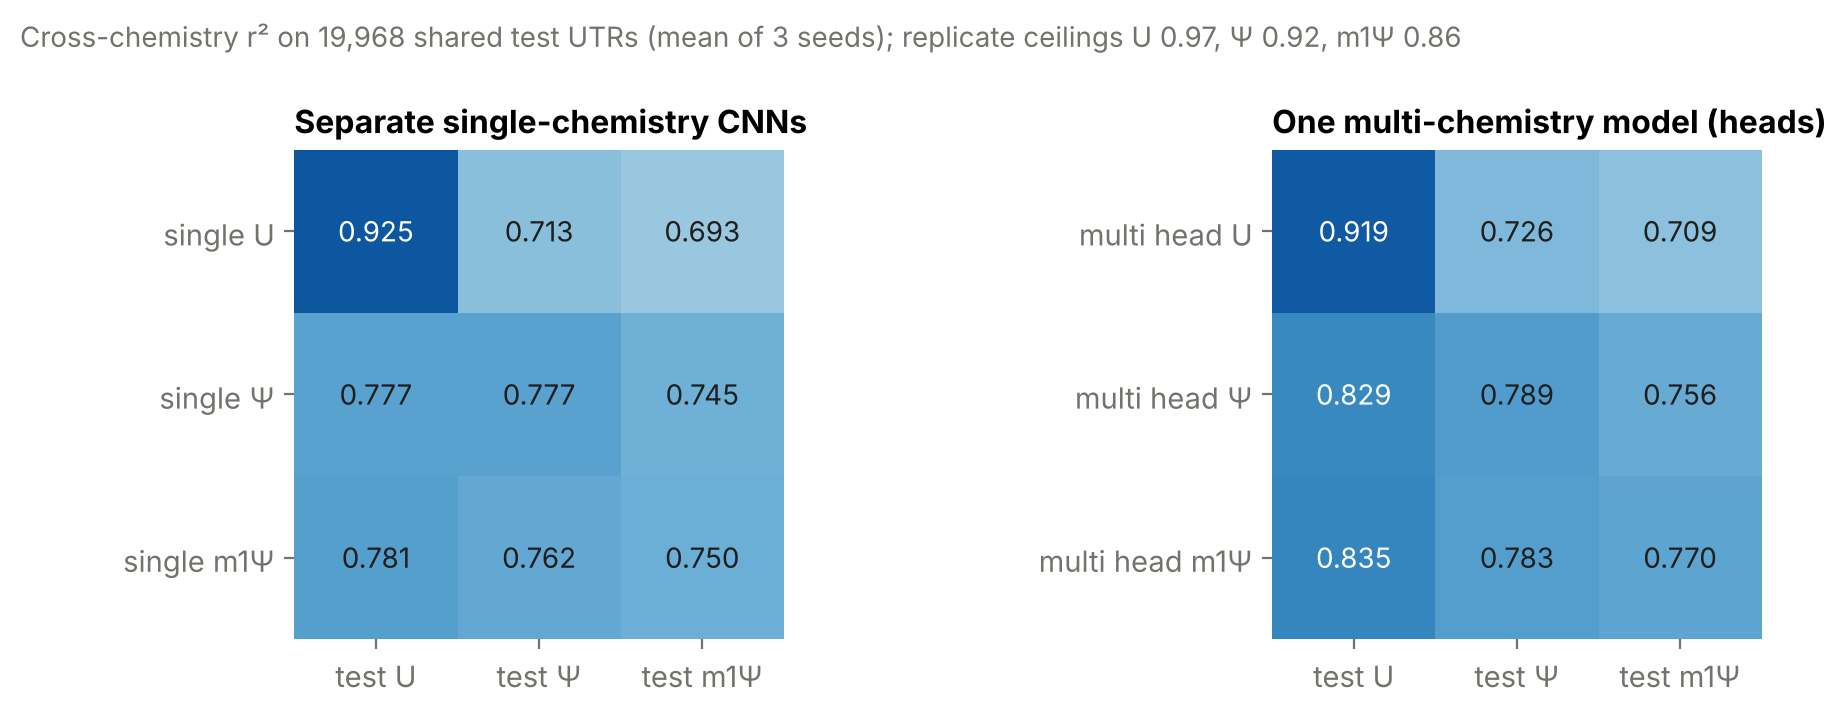
\includegraphics[width=\textwidth]{figs/A_cross_chemistry.png}
\caption{Cross-chemistry $r^2$ on the 19{,}968 shared test UTRs (mean of three seeds). Rows
are the training chemistry (left) or the output head (right); columns are the evaluation
labels. One shared model improves the modified chemistries on the diagonal and transfers
markedly better off-diagonal.}
\label{fig:chem}
\end{figure*}

The original work trains a separate network per chemistry, which cannot exploit the fact
that the same 280{,}000 sequences are measured in all three. We train one model with a
shared CNN trunk and chemistry conditioning, comparing two conditioning schemes on the
validation split: a learned chemistry embedding concatenated to the representation, versus
separate output heads. Separate heads won narrowly (mean validation $r^2$ 0.6705 vs.\
0.6677) and are used throughout. Labels are masked where missing, so a sequence contributes
to whichever chemistries measured it.

Results are in Figure~\ref{fig:chem}. The shared model improves m1$\Psi$ from
$0.750 \pm 0.010$ to $0.770 \pm 0.008$ (better in 3/3 seeds) and $\Psi$ from
$0.777 \pm 0.005$ to $0.789 \pm 0.009$ (2/3 seeds), at a cost of 0.006 on U. The larger
effect is off-diagonal: the $\Psi$ and m1$\Psi$ \emph{heads} predict U labels at
$r^2 \approx 0.83$, whereas separately trained $\Psi$/m1$\Psi$ models manage 0.78. The shared
trunk carries information learned from the abundant U data into the modified-chemistry
heads. As noted above, the multi-task model is worse calibrated and benefits from a
validation-fitted linear correction.

\subsection{Architectures across data regimes}
\label{sec:arch}

\begin{figure}[t]
\centering
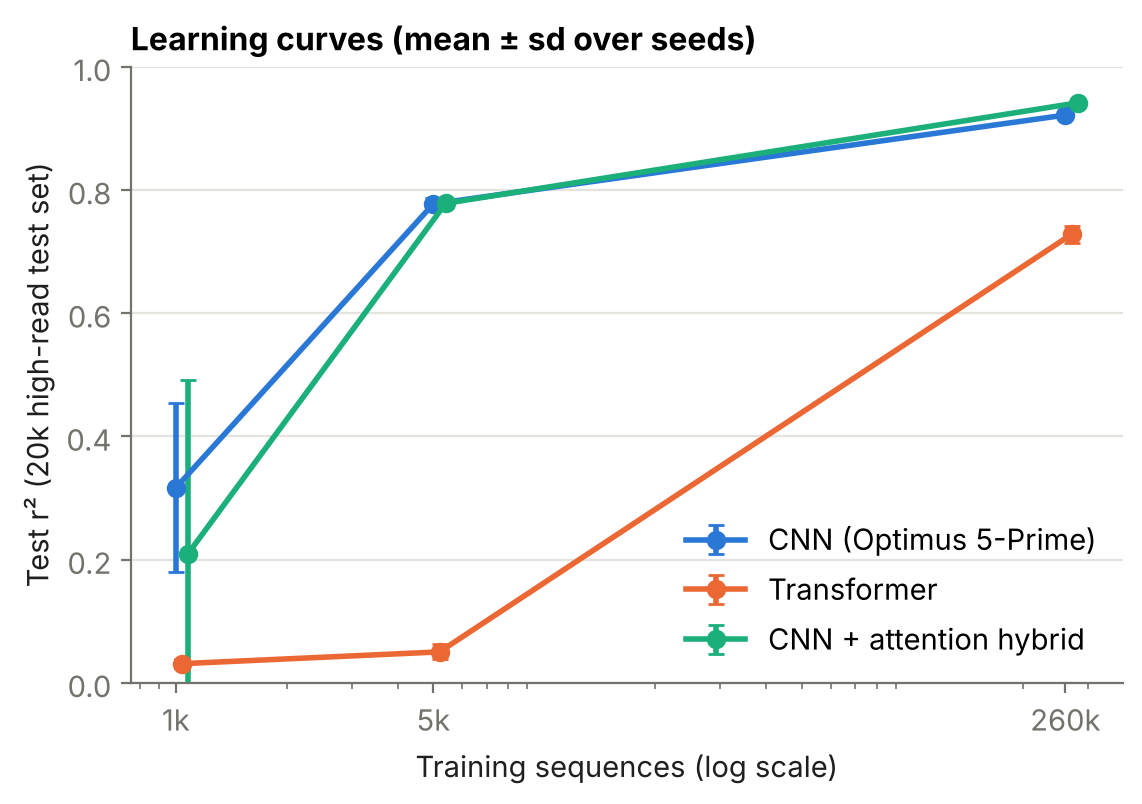
\includegraphics[width=\columnwidth]{figs/B_learning_curves.png}
\caption{Learning curves. Parameter counts are matched (475k / 457k / 421k) and every
architecture receives the same tuning budget, early-stopping rule and seeds at each data
size. The transformer's full-data point is budget-limited (see text).}
\label{fig:lc}
\end{figure}

The paper evaluates one architecture at one data size. We compare three at
$\{1\mathrm{k}, 5\mathrm{k}, 260\mathrm{k}\}$ training sequences: the CNN (475k parameters),
a pre-LN transformer encoder~\citep{vaswani2017} over the 50 positions with learned
positional embeddings and mean pooling (457k), and a hybrid of two convolutional layers feeding a three-layer
transformer (421k). Fairness controls: matched parameter counts, an identical tuning grid
per architecture per data size (learning rate $\times$ dropout, selected on validation),
the same early-stopping rule, five seeds at 1k/5k and three at full data, and nested random
subsets drawn only from the training pool.

\begin{table}[t]
\caption{Test $r^2$ by architecture and training-set size (mean $\pm$ sd; five seeds at
1k/5k, three at 260k). $^\dagger$All three full-data transformer runs hit the 15-epoch cap
while validation loss was still falling, so this value is budget-limited rather than a
converged ceiling.}
\label{tab:arch}
\vskip 0.1in
\begin{center}
\begin{small}
\begin{tabular}{lccc}
\toprule
Train size & CNN & Transformer & Hybrid \\
\midrule
1{,}000   & $\mathbf{0.317}${\scriptsize$\pm.123$} & $0.031${\scriptsize$\pm.007$} & $0.210${\scriptsize$\pm.251$} \\
5{,}000   & $\mathbf{0.778}${\scriptsize$\pm.009$} & $0.050${\scriptsize$\pm.011$} & $\mathbf{0.778}${\scriptsize$\pm.005$} \\
260{,}000 & $0.922${\scriptsize$\pm.002$} & $0.728^\dagger${\scriptsize$\pm.012$} & $\mathbf{0.942}${\scriptsize$\pm.001$} \\
\bottomrule
\end{tabular}
\end{small}
\end{center}
\vskip -0.1in
\end{table}

Table~\ref{tab:arch} and Figure~\ref{fig:lc} give the result. \textbf{The hybrid is the best
model at full data}, reaching $r^2 = 0.942 \pm 0.001$ --- above the published CNN on all
three seeds, with fewer parameters and lower RMSE (0.454 vs.\ 0.522). The convolutional stem
supplies the local motif prior that attention otherwise has to discover, while self-attention
adds the long-range composition the CNN lacks.

\textbf{The pure transformer fails, and the failure is informative.} At 1k and 5k it cannot
fit even its training set. We verified this is not an implementation bug using training data
only: changing the learning rate does not help, replacing the learned positional embedding
with a sinusoidal one does not help, and the identical encoder behind a convolutional stem
(the hybrid) trains normally. At full data it sits on a plateau for roughly eight epochs
($\approx14$k updates) before breaking out, and all three runs were stopped by the shared
15-epoch cap while still improving. Learning a motif such as ATG from single-nucleotide
tokens through attention alone requires far more optimisation steps than the convolutional
prior needs.

\paragraph{Sensitivity and controls.} Because the hybrid is bimodal at 1k (either
$\approx0.65$ or $\approx0.04$, depending on whether it escapes the initial plateau), we
repeated the small-data runs with patience 30 instead of 10 for \emph{all} architectures.
This lifts the CNN at 1k from 0.317 to $0.435 \pm 0.054$ --- the shared rule was
under-training the CNN too --- but does not rescue the transformer (0.035) nor remove the
hybrid's bimodality, and the ranking at 5k is unchanged. On a random (rather than
read-depth) test split, single-seed full-data scores are CNN 0.891 and hybrid 0.896 versus
0.923 and 0.941 on the high-read split: the modest drop is expected since random test sets
include noisier low-coverage UTRs, and the ordering holds.

\subsection{Cross-chemistry transfer}

\begin{figure*}[t]
\centering
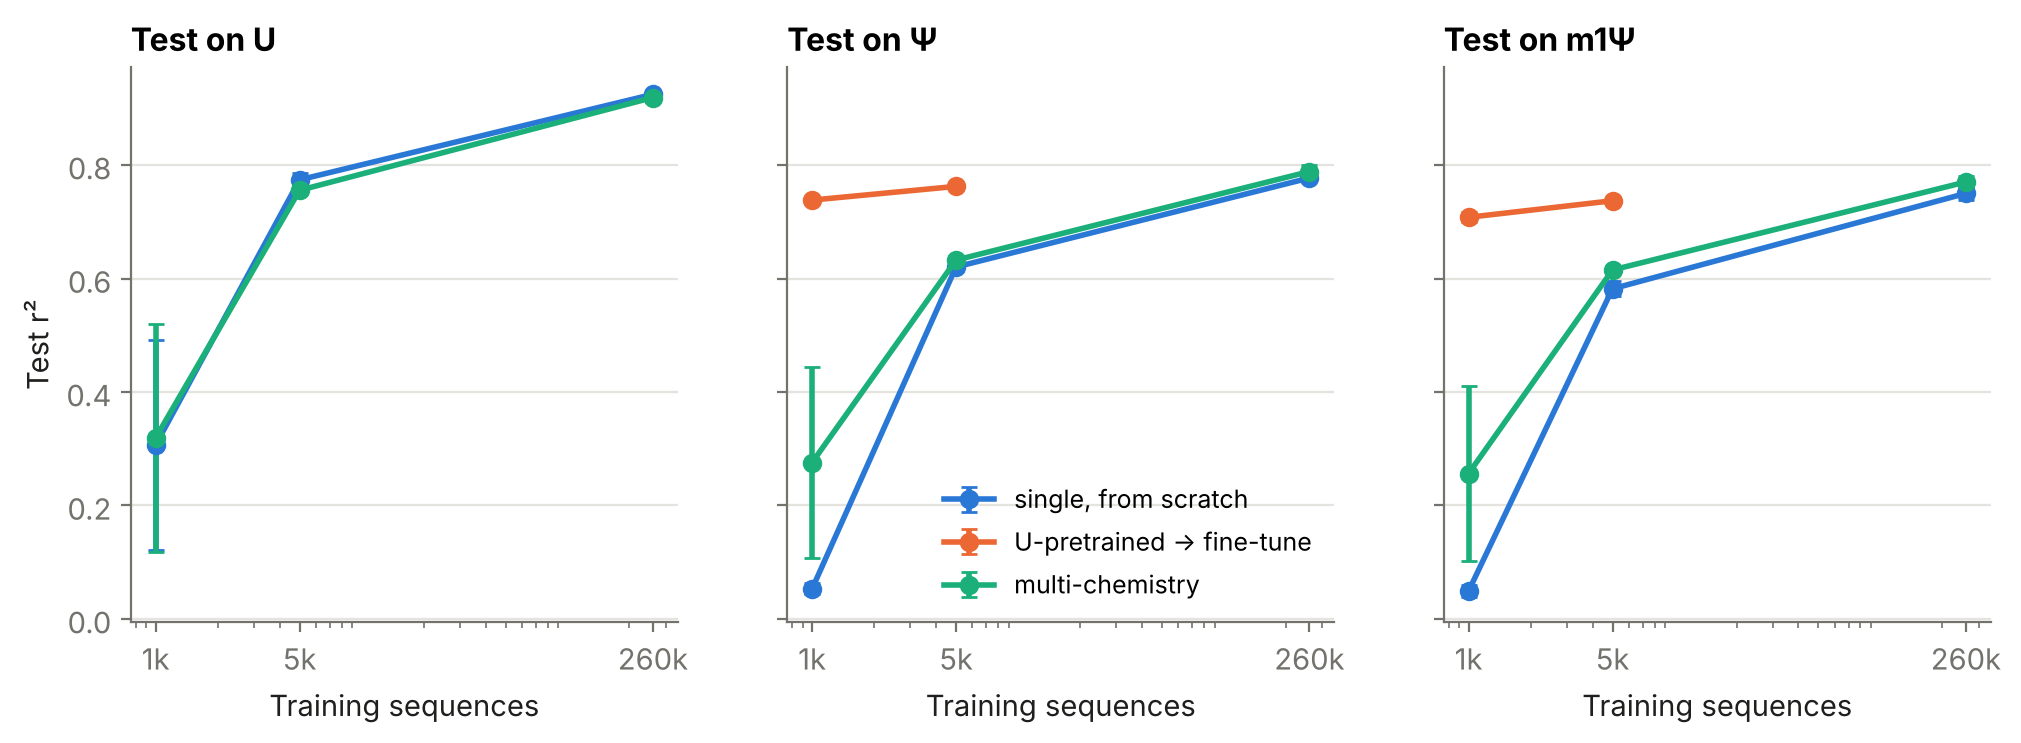
\includegraphics[width=\textwidth]{figs/B_chemistry_regimes.png}
\caption{Training-set size versus test $r^2$ for each chemistry. Fine-tuning a model
pre-trained on unmodified RNA recovers most of the full-data performance from 1{,}000
modified-chemistry sequences.}
\label{fig:regimes}
\end{figure*}

Modified-nucleotide libraries are expensive, so the practical question is how little
modified-chemistry data is needed. We compare, at matched budget, training from scratch,
fine-tuning a U-pretrained CNN, and the multi-task model (Figure~\ref{fig:regimes}).
The effect is large: with \textbf{1{,}000} $\Psi$ sequences, fine-tuning reaches
$r^2 = 0.738 \pm 0.003$ where from-scratch training manages $0.053 \pm 0.008$ --- 95\% of
the performance of a model trained on the full 260{,}000 ($0.777$). With 5{,}000 sequences,
fine-tuning ($\Psi$ 0.762, m1$\Psi$ 0.737) matches or exceeds from-scratch training on
260{,}000 for m1$\Psi$ (0.750). For a laboratory, this converts a full MPRA into a small
calibration experiment.

\subsection{Variant effect prediction}

\begin{figure*}[t]
\centering
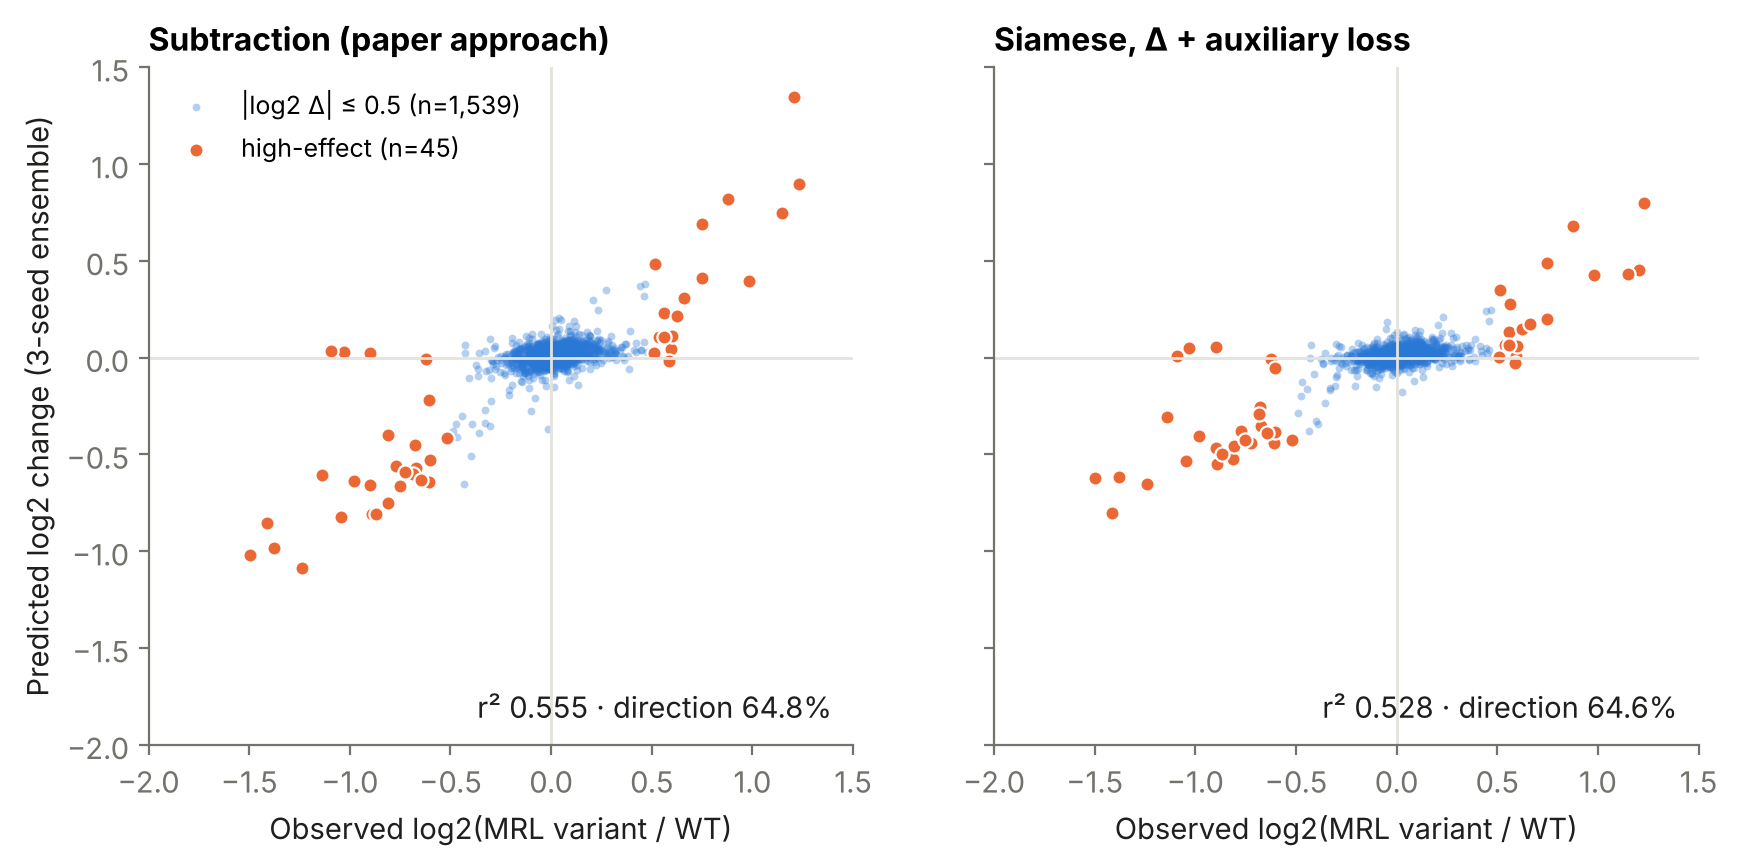
\includegraphics[width=0.86\textwidth]{figs/C_variant_effects.png}
\caption{Predicted vs.\ observed $\log_2$ MRL change for 1{,}584 ClinVar 5$'$UTR variants,
pooled out-of-fold over wild-type-grouped cross-validation. The learned paired model (right)
does not improve on subtraction (left).}
\label{fig:variant}
\end{figure*}

The paper predicts a variant's effect by predicting wild-type and variant MRL independently
and subtracting, achieving $r^2 = 0.555$. We asked whether a model trained directly on the
difference does better. We built a Siamese architecture sharing an encoder over both
sequences, with a head on $[\mathbf{h}_{\text{var}} - \mathbf{h}_{\text{wt}},\,
\mathbf{h}_{\text{wt}} \odot \mathbf{h}_{\text{var}}]$ predicting
$\log_2(\mathrm{MRL}_{\text{var}} / \mathrm{MRL}_{\text{wt}})$, optionally with an auxiliary
loss on both absolute MRLs. Training pairs include 5{,}519 single-nucleotide
synthesis-error pairs as additional supervision.

\paragraph{Leakage control.} Variants of the same wild-type sequence are highly correlated,
so random pair splits leak. We assign folds by \emph{connected component}: any two sequences
linked through any pair fall in the same fold. We verified that no sequence appears in more
than one fold.

\begin{table}[t]
\caption{Variant-effect prediction on 1{,}584 ClinVar pairs (45 with
$|\log_2\Delta|>0.5$), pooled out-of-fold, mean $\pm$ sd over three seeds. ``Dir.'' is sign
agreement. The paper's reported 76\% for high-effect variants is an $r^2$, not an accuracy.}
\label{tab:variant}
\vskip 0.1in
\begin{center}
\begin{small}
\setlength{\tabcolsep}{4pt}
\begin{tabular}{lccc}
\toprule
Method & $r^2$ & Dir. & $r^2_{\text{high}}$ \\
\midrule
Paper (as stated) & 0.555 & 64\% & 0.76 \\
Authors' released predictions & 0.553 & 65.1\% & 0.762 \\
\midrule
Subtraction (ours) & $0.540${\scriptsize$\pm.005$} & 64.6\% & 0.771 \\
\quad + fine-tune on human MRLs & $0.544${\scriptsize$\pm.006$} & 64.1\% & \textbf{0.778} \\
Siamese on $\Delta$ & $0.477${\scriptsize$\pm.009$} & 60.6\% & 0.749 \\
Siamese + auxiliary loss & $0.495${\scriptsize$\pm.009$} & 62.4\% & 0.744 \\
\bottomrule
\end{tabular}
\end{small}
\end{center}
\vskip -0.1in
\end{table}

\textbf{This extension is a negative result} (Table~\ref{tab:variant},
Figure~\ref{fig:variant}). The Siamese model is worse than subtraction on $r^2$ and on
direction accuracy, and only ties on AUROC for identifying large-effect variants. Fine-tuning
the encoder on in-domain human MRLs before subtracting also does not help ($+0.004$, within
noise). Our interpretation: a CNN trained on 260{,}000 random sequences already encodes the
relevant grammar, and $\approx$5{,}000 noisy measured differences are too few and too noisy
to improve on it. Subtraction alone reproduces the published number
(three-seed ensemble: $r^2 = 0.555$).

\paragraph{Saturation mutagenesis.} We scored all 150 single-nucleotide substitutions of the
CPOX, TMEM127 and RPL5 5$'$UTRs. Subtraction ranks each highlighted ClinVar variant as the
\emph{single most MRL-reducing} substitution in its UTR (CPOX G$-$10A, observed $-0.89$,
predicted $-0.81$; TMEM127 C$-$18T, $-1.50$/$-1.02$; RPL5 C$-$46A, $-0.87$/$-0.81$), while
the two other alleles at RPL5 position $-46$ are correctly predicted near-neutral (ranks 90
and 53 of 150). This reproduces the paper's Figure~4c qualitatively and exactly.

\subsection{Attribution and motif discovery}

\begin{figure*}[t]
\centering
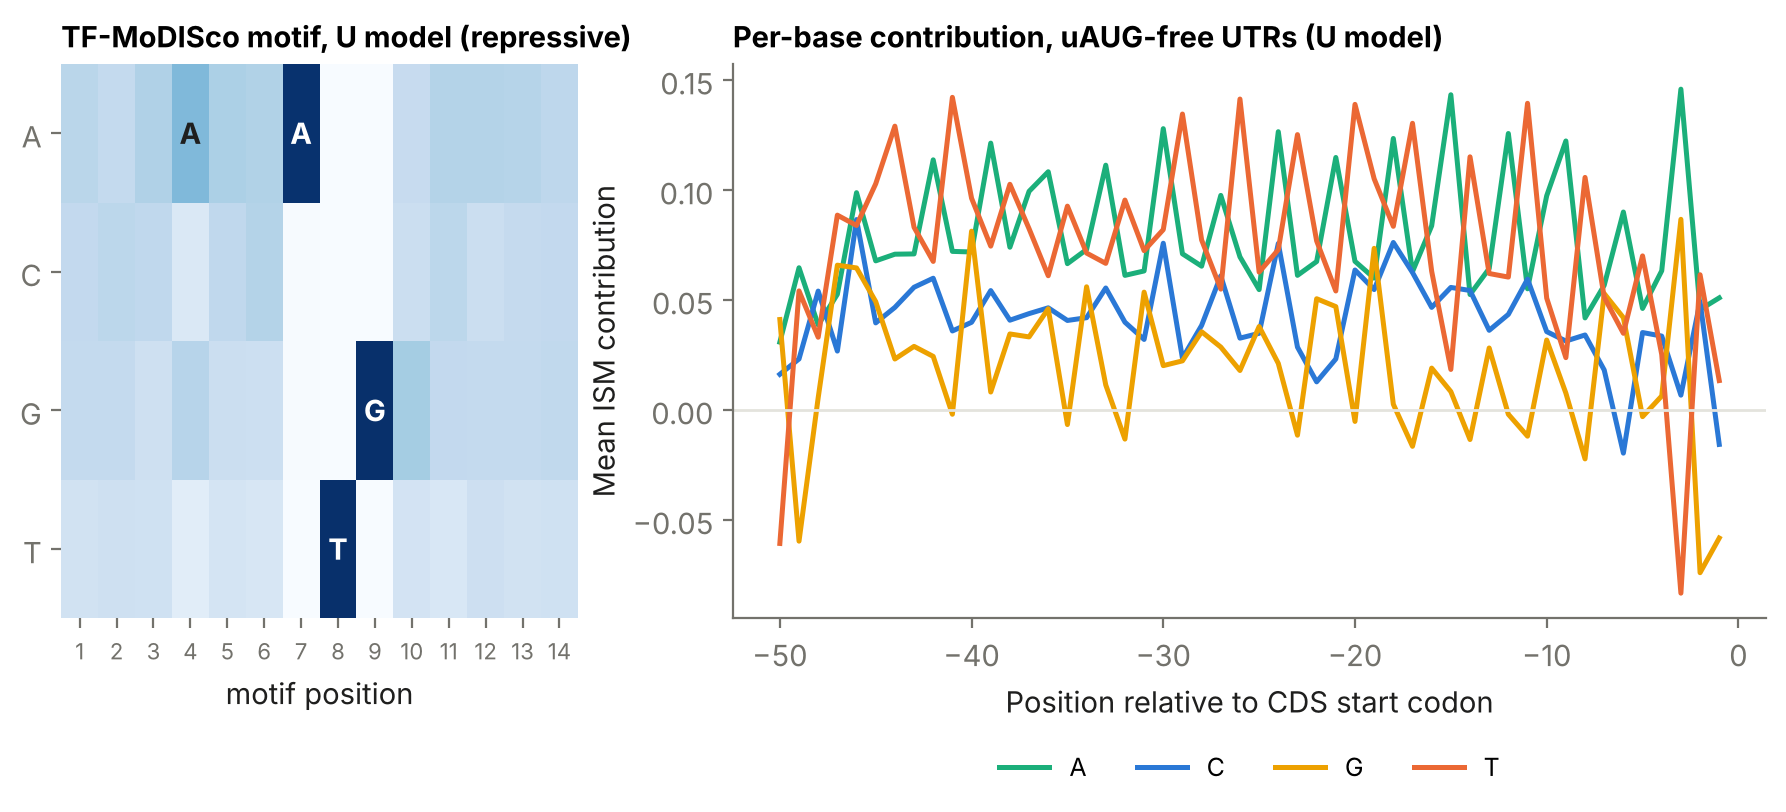
\includegraphics[width=\textwidth]{figs/D_motif_and_profile.png}
\caption{Left: the single repressive motif recovered \emph{de novo} by TF-MoDISco from the
unmodified-RNA model --- an upstream AUG in Kozak-like context. Right: mean per-base ISM
contribution by position in uAUG-free UTRs, showing the Kozak $-3$ purine preference near
the CDS.}
\label{fig:motif}
\end{figure*}

We applied integrated gradients~\citep{sundararajan2017} (uniform baseline, 32 steps; completeness error
$<5\times10^{-4}$) and exhaustive single-nucleotide in-silico mutagenesis (ISM) to 2{,}000
shared test UTRs.

\textbf{Motifs.} TF-MoDISco~\citep{shrikumar2018} recovers exactly one repressive motif for every chemistry, with
consensus \texttt{AAAAATGG} (589--678 seqlets): an upstream AUG with an A-rich upstream
context and G at $+4$ --- the Kozak context, learned \emph{de novo}
(Figure~\ref{fig:motif}). Restricting to the 602 uAUG-free UTRs, so that uAUGs do not
dominate, enrichment analysis finds GC-rich pentamers (\texttt{GCCCG}, \texttt{CCCCG}) as
repressive, consistent with structure, and a purine-rich \texttt{AAGGA}/\texttt{TAAGG}
element as activating at any position. The latter matches no element in our curated list
(Kozak, uAUG, stops, CUG/GUG, GC/AU-rich, ARE, Pumilio, poly-U, G-runs); we flag it as
unmatched rather than claim a discovery, noting that no offline RBP motif database was
available to us. The per-position profile independently recovers the Kozak $-3$ purine rule
at the main start codon.

\textbf{CNN vs.\ attention.} The hybrid's ISM maps agree with the CNN's at per-sequence
$r = 0.96$ with 84\% overlap in top-5 attributed positions --- nearly as close as two CNN
seeds agree with each other ($r = 0.97$). The hybrid therefore wins by refining a shared
grammar, not by learning a different one. The pure transformer agrees less ($r = 0.79$,
64\% overlap) and relies less on uAUGs. We note that integrated-gradients agreement is much
lower than ISM agreement across architectures (e.g.\ 0.30 for CNN vs.\ transformer), so we
treat ISM as the more stable comparison.

\textbf{A negative result on the structure hypothesis.} \citet{sample2019} report that MRL
correlates more strongly with MFE for modified chemistries ($r = 0.43$, 0.56, 0.58 for U,
$\Psi$, m1$\Psi$). On uAUG-free test UTRs we measure 0.437, 0.433 and 0.439: U matches
exactly, but we see no increase for the modified chemistries. Our models do rely less on
uAUGs for modified RNA (an ATG-creating substitution changes predictions by $-1.12$, $-0.81$,
$-0.78$ in standardised units), and GC sensitivity relative to that uAUG effect rises
slightly (0.040, 0.042, 0.046), which is directionally consistent but far weaker than the
published claim. The exact MFE protocol of the original work is not specified, so a
methodological difference cannot be excluded.

\section{Discussion and Limitations}

Our strongest positive results are the hybrid architecture ($+0.020$ $r^2$ over the published
CNN, consistent across seeds) and cross-chemistry transfer (95\% of full-data performance
from 1{,}000 sequences). Both have direct practical value for mRNA design. The
chemistry-conditioned model is a smaller but real gain, and it comes with a calibration
caveat we would have missed had we reported only $r^2$.

Several limitations should be stated plainly. \textbf{Compute.} All experiments ran on two
CPU cores without a GPU, which forced a 15-epoch cap at full data. The transformer in
particular was still improving when stopped, so its ceiling is unknown, and the hybrid's
margin over the CNN is established only within that shared budget. \textbf{Variance at small
data.} At 1k the hybrid is bimodal and standard deviations are large; conclusions there are
about typical-case behaviour under a fixed budget, not about asymptotic capacity.
\textbf{Chemistry scope.} Human and ClinVar libraries were measured only in unmodified RNA
--- we verified this from the data itself, since the designed library's control UTRs agree
with U at $r^2$ 0.86/0.80 versus 0.45--0.64 for the modified chemistries --- so all
variant-effect results are U-only and no multi-chemistry claim is made there.
\textbf{Motif novelty.} The unmatched purine-rich element is flagged, not claimed; testing it
against a proper RBP database is the obvious next step.

\section{Conclusion}

We reproduced Optimus 5-Prime faithfully, validated the pipeline on a synthetic dataset with
known rules, and benchmarked it against three alternatives with both regression and
classification metrics. Four extensions followed: a chemistry-conditioned multi-task model, a
CNN+attention hybrid that improves on the published architecture, a transfer study that makes
modified-chemistry modelling cheap, and an attribution analysis that recovers the Kozak-context
uAUG motif \emph{de novo}. We report in equal detail the two extensions that did not work ---
the Siamese variant-effect model and the secondary-structure chemistry hypothesis --- because
a reproduction study whose every extension succeeds is not a reproduction study.

\section*{Code and Reproducibility}
All code, trained weights, per-run metrics (including validation curves and seeds), saved
subset indices, and the scripts that regenerate every figure and table in this report are at
\url{\repourl}. A one-minute demonstration script
(\texttt{python3 demo.py}) reproduces the headline numbers from shipped weights and runs a
live 5{,}000-sequence training job.

\section*{Author Contributions}
\textit{Tushar Srikrishna Sridhar (231103), Anika Gupta (230137) and Prutha Vinay (230807)
contributed to this project. Specific contributions to be filled in by the group.}

\bibliography{refs}
\bibliographystyle{icml2026}

\end{document}
